\documentclass[border=5mm]{standalone}
\usepackage{tikz}
\usetikzlibrary{matrix, positioning, arrows.meta}

\begin{document}
	

		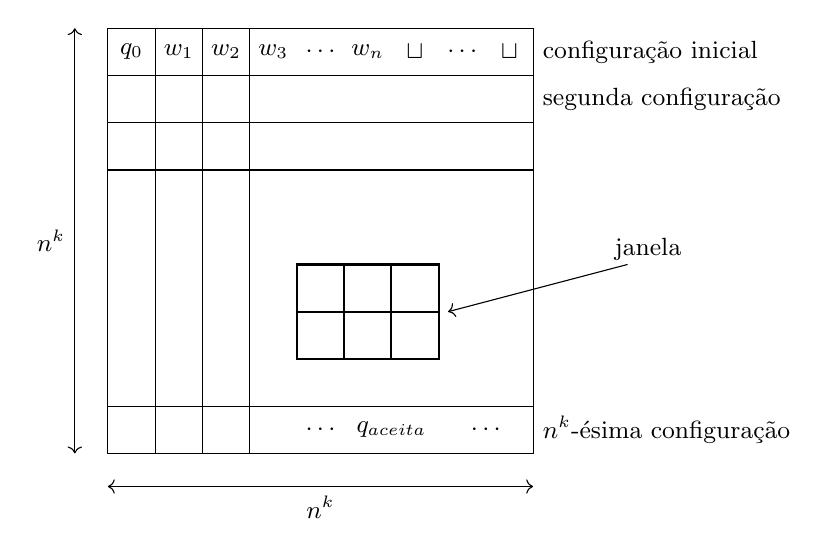
\begin{tikzpicture}[scale=0.6, every node/.style={font=\small, anchor=center}]

			
			% Grade principal
			\foreach \i in {1,...,3} {
				\foreach \j in {1,8,9} {
					\draw (\i,\j) rectangle ++(1,1);
				}
			}
			
			\foreach \i in {1,2,3,4}{ \foreach \j in {1,8,9}{\draw (\i,\j) rectangle (1,1);}}
			
			\foreach \i in {2,7,8,9,10}{ \foreach \j in {10}{\draw (\j,\i) rectangle (1,1);}}
			
		
			
			
			% Configuração inicial (linha do topo, y = nk)
			\node at (1.5, 9.5) {$q_0$};
			\node at (2.5, 9.5) {$w_1$};
			\node at (3.5, 9.5) {$w_2$};
			\node at (4.5, 9.5) {$w_3$};
			\node at (5.5, 9.5) {$\cdots$};
			\node at (6.5, 9.5) {$w_n$};
			\node at (7.5, 9.5) {$\sqcup$};
			\node at (8.5, 9.5) {$\cdots$};
			\node at (9.5, 9.5) {\(\sqcup\)};
			\node at (5.5,1.5) {\(\cdots\)};
			\node at (7,1.5) {\(q_{aceita}\)};
			\node at (9,1.5) {\(\cdots\)};
			
			
			% Janela 3x2 no centro
			\foreach \i in {3,4} {
				\foreach \j in {5,6,7} {
					\draw[thick] (\j, \i) rectangle ++(1,1);
				}
			}
			
			% Anotações de configuração
			\node[anchor=west] at (10, 9.5) {configuração inicial};
			\node[anchor=west] at (10, 8.5) {segunda configuração};
			\node[anchor=west] at (10, 1.5) {\(n^k\)-ésima configuração};
			
			% Seta para a janela
			\draw[->] (12, 5) -- (8.2, 4) node[very near start,above right] {janela};
			
			% Setas de dimensão
			\draw[<->] (0.3, 1) -- (0.3, 10) node[midway, left] {\(n^k\)};
			\draw[<->] (1, 0.3) -- (10, 0.3) node[midway, below] {\(n^k\)};
			
		\end{tikzpicture}
\end{document}
